In 1962, game developers wrote code that directly controlled individual pixels. \emph{Spacewar!} on the PDP-1 computed each dot's position through direct arithmetic: $x + dx$, $y + dy$. The electron beam drew vectors where the calculations specified. No abstraction layers existed between the programmer's calculations and the phosphor display. Each spaceship consisted of six numbers in memory — position, velocity, angle, and fuel. The game loop ran sixty times per second: read switch states from the control panel, update positions by adding velocities, subtract fuel for thrust, apply gravity as a constant acceleration toward the center, check if position vectors intersected for collisions, then send the computed coordinates to the vector display. The entire program fit in 4K of memory.

Early arcade machines hardcoded every behavior into separate routines. \emph{Space Invaders} (1978) implemented each alien type with its own movement function, its own collision detection, its own point calculation. Moving the bottom row required one function that decremented x-coordinates and checked the left boundary. Moving the middle row used a different function with different speed constants. The top row had its own handler. When any alien touched the screen edge, specific code executed to move all aliens down one row and reverse the direction flag. Adding a new enemy type meant writing new functions for movement, new functions for collision detection, new functions for scoring — touching every system in the game. The code grew linearly with content.

Programmers began utilizing these patterns of repetition. Every moving object needed position and velocity. Every visible object needed drawing routines. Every destructible object needed health values. In \emph{Adventure} (1979), Warren Robinett faced the Atari 2600's 128 bytes of RAM. He couldn't afford separate code for each object type. Instead, he consolidated repeated elements into a single object handler. Dragons, bats, keys, and swords were entries in an object table, each storing position, size, color, and a behavior ID. The behavior ID indexed into a jump table of function pointers. Object \texttt{0x1A} (the yellow key) had behavior type \texttt{0x04} (can be picked up). Object \texttt{0x0E} (the red dragon) had behavior type \texttt{0x07} (chase player). One collision detection routine handled all interactions by comparing behavior IDs. One drawing routine rendered all objects by reading their size and color. 

 When Toru Iwatani designed \emph{Pac-Man} (1979), he gave all four ghosts the same movement code but different target selection algorithms. Blinky (red) targeted Pac-Man's current tile. Pinky (pink) targeted four tiles ahead of Pac-Man in his facing direction. Inky (cyan) computed a complex target: take the position two tiles in front of Pac-Man, draw a vector from Blinky to that position, then double it. Clyde (orange) chased Pac-Man when more than eight tiles away but fled to his home corner when closer. Four ghosts from one movement function with different target coordinates.

The 1990s brought object-oriented programming to game development. \emph{Doom} (1993) structured its actors through inheritance hierarchies. Every monster derived from a common base class containing position, health, and state machine logic. The imp and the baron of hell executed identical state machine code. They differed only in their data tables: health points (60 versus 1000), projectile type (fireball versus plasma ball), movement speed (8 versus 8 units per tic), pain chance (200/256 versus 50/256). State machines were data. The imp's fireball attack was state S\_TROO\_ATK3: display sprite TROOF, duration 8 tics, action function A\_TroopAttack, next state S\_TROO\_1. New monsters by mixing existing action functions with new sprites and parameters. The Revenant combined A\_SkelMissile (fire homing missile) with A\_SkelFist (punch if close). The Archvile combined A\_VileChase (resurrect dead monsters) with A\_VileAttack (immolating flame attack). No new code required — just new data tables.

By 2000, inheritance hierarchies had limitations. A FlyingEnemy class couldn't share code with a FlyingProjectile without multiple inheritance. A FireGolem pulled from both Golem and FireCreature, creating diamond inheritance – when a class inherits from two classes that inherit from the same class. Deep hierarchies were fragile. changing Animal broke Dog which broke FlyingDog which broke FireBreathingFlyingDog. Entity-component systems replaced them. An entity was just an ID number. Components were bags of data: \texttt{Position \{x: 5, y: 10, z: 3\}}, \texttt{Velocity \{dx: 1, dy: 0, dz: 0\}}, \texttt{Sprite \{texture: "goblin.png"\}}, \texttt{Health \{current: 30, max: 30\}}, \texttt{AI \{behavior: "aggressive"\}}. Systems were functions that processed components. MovementSystem iterated through all entities with Position and Velocity, updating positions. RenderSystem drew all entities with Position and Sprite. DamageSystem processed collisions for entities with Health. Adding flight to a goblin meant adding a Flying component. Making a barrel explode meant adding an Explosive component. A flying, exploding, invisible barrel needed no new class — just combine Flying, Explosive, and remove the Sprite component.

Game engines were standardized architectures. id Tech, Unreal Engine, and Unity provided complete frameworks: rendering pipelines with shaders and occlusion culling, physics engines with collision detection and constraint solvers, audio systems with 3D spatialization, networking layers with client prediction and lag compensation. Developers no longer built engines from scratch. They configured existing systems, wrote gameplay scripts, created art assets.  A game was configuration data plus custom logic, running on someone else's foundation. Most games using these engines still required teams of specialists to craft specific experiences. Some games took a different approach: providing tools for players to build their own content within the game's systems.

\emph{Minecraft} used these principles extensively. Markus Persson wrote no hardcoded mining animations, no specific crafting sequences, no predetermined progression. He built basic systems: Blocks had properties: hardness, tool requirements, light emission, update behaviors. Items had functions: dig block, place block, damage entity. Entities had composable AI tasks.  Place blocks, break blocks, update neighbors. Players built cities, computers, musical instruments, working calculators. Redstone dust carried signals up to 15 blocks. Torches inverted signals — powered input produced unpowered output. Repeaters delayed signals by 1-4 ticks. Pistons pushed blocks when powered. Players built logic gates: NOT gates from single torches, OR gates from merged dust lines, AND gates from torch arrays, memory cells from piston feedback loops.  Players built 8-bit CPUs, graphing calculators, playable musical instruments.  The programmer set the stage, the players set the game.

Entities in \emph{Minecraft} used composition. The base Entity class defined position, velocity, and bounding box. LivingEntity added health and damage handling. Mob added a list of AI tasks, small behavior programs that executed each tick. Tasks were objects with simple interfaces: \texttt{shouldExecute()} to check if the task should run, \texttt{startExecuting()} to initialize, \texttt{updateTask()} to perform the behavior. A zombie's task list contained \texttt{AttackPlayerTask} (priority 2), \texttt{WanderTask} (priority 5), \texttt{LookAtPlayerTask} (priority 8). A sheep had \texttt{EatGrassTask}, \texttt{FollowParentTask}, \texttt{PanicTask}.  The cow was wander + follow player holding wheat + panic when hurt. The skeleton was attack player + flee from wolves + avoid sunlight. Every mob assembled from the same components.

Among these assembled creatures was the Creeper — \emph{Minecraft}'s most recognizable enemy. Silent, green, explosive. It approaches players without warning and detonates on proximity, destroying carefully built constructions. Unlike zombies that moan or skeletons that rattle, the Creeper moves in complete silence until its final hiss. No other mob behaves like it. The Creeper began as a pig. In 2009, Persson was implementing farm animals and creating a pig model. In his 3D modeling program, he entered the creature's dimensions. The pig required length 2.0, height 1.0, width 1.0 — a horizontal rectangle with stubby legs. But when typing the values, Persson accidentally swapped length and height, entering height 2.0, length 1.0. Instead of a quadruped, he got a vertical pillar with four tiny legs at the bottom. The model file loaded without error — \emph{Minecraft}'s model loader accepted any valid vertex data. The renderer displayed exactly what it received: a tall, thin creature standing upright. Persson found the error amusing. He textured it green using the same grass texture used for blocks, added a frowning mouth, adjusted the legs to look more like feet. He kept it as a joke, then made it explode. He copied TNT's explosion code — remove blocks within radius R, damage entities by inverse square distance, spawn item entities for destroyed blocks. He bound this to proximity detection borrowed from zombie AI: if distance to player less than 3 blocks, start countdown timer. After 1.5 seconds, detonate. No footstep sounds were assigned because pigs didn't have footsteps yet.

\textbf{Street Fighter II} (1991) had combos through a programming oversight. During development, producer Noritaka Funamizu discovered that the recovery time after certain moves was shorter than the hit-stun inflicted on opponents. By timing inputs precisely, players could land a second attack before the opponent recovered from the first. The window was narrow — frame-perfect in some cases — and the developers assumed players would rarely exploit it. But location test players began discovering two-hit and three-hit sequences. Capcom watched players develop increasingly complex chains: jump kick into standing fierce into special move. Instead of patching the timing windows, they kept it.  Every subsequent fighter implemented deliberate combo systems with cancels, links, and chains.

\textbf{Quake} (1996) introduced rocket jumping through physics engine oversight. The game calculated explosion damage and knockback for all entities within the blast radius — including the player who fired the rocket. Players discovered that firing at their feet while jumping added the explosion's upward force to their jump velocity, reaching otherwise inaccessible platforms. The technique required precise timing and cost health, creating risk-reward gameplay.  \textbf{Grand Theft Auto} began development as \emph{Race'n'Chase}, a straight racing game with police chases. During testing, a quirk of the police AI made them impossibly aggressive. Instead of trying to box players in, they rammed at full speed.  Testers found themselves spending more time fleeing from psychotic police than racing. The chaotic pursuits were more entertaining than the intended gameplay. DMA Design redesigned the entire game around the bug. Racing became secondary to mayhem.

\textbf{Devil May Cry} (2001) originated from a scrapped \emph{Resident Evil 4} prototype. The prototype's combat engine felt too fast and stylish for a survival horror game. Capcom spun it into a new IP focused on the combat mechanics. \emph{Devil May Cry} rated players on combo variety, introduced air launches, wall running, and gun juggling.

\textbf{Space Invaders} (1978) had increasing difficulty through hardware limitations. Tomohiro Nishikado programmed the aliens to move at constant speed, but the Intel 8080 processor couldn't maintain consistent frame rates. With 55 aliens on screen, the game ran slowly. As players destroyed aliens, the processor had fewer sprites to update, causing the remaining aliens to move faster.  Nishikado kept the unintended acceleration.

\textbf{Tribes} (1998) had movement physics bugs. Players discovered that rapidly tapping jump while descending slopes prevented the normal friction from applying. Each jump reset the friction calculation before it could slow the player. This "skiing" technique allowed tremendous speed, changing combat speed. Dynamix kept it, designing maps with long slopes, adding routes specifically for skiing, balancing weapons around high-speed combat.

\textbf{Silent Hill} (1999) used fog to hide hardware limitations. The PlayStation couldn't render distant polygons without severe popup and texture warping. Instead of reducing draw distance with traditional fog walls, Team Silent implemented thick, volumetric fog that moved and swirled.  The fog hid threats and masked jump scares.

\textbf{Super Smash Bros. Melee} (2001) had physics oversights. Wavedashing happened when air dodging diagonally into the ground. Air dodging diagonally into the ground preserved momentum while landing, causing characters to slide. Players could attack while sliding, opening new approach options. Nintendo never intended wavedashing — Masahiro Sakurai called it an exploit. 

\vspace{2em}
\begin{center}
    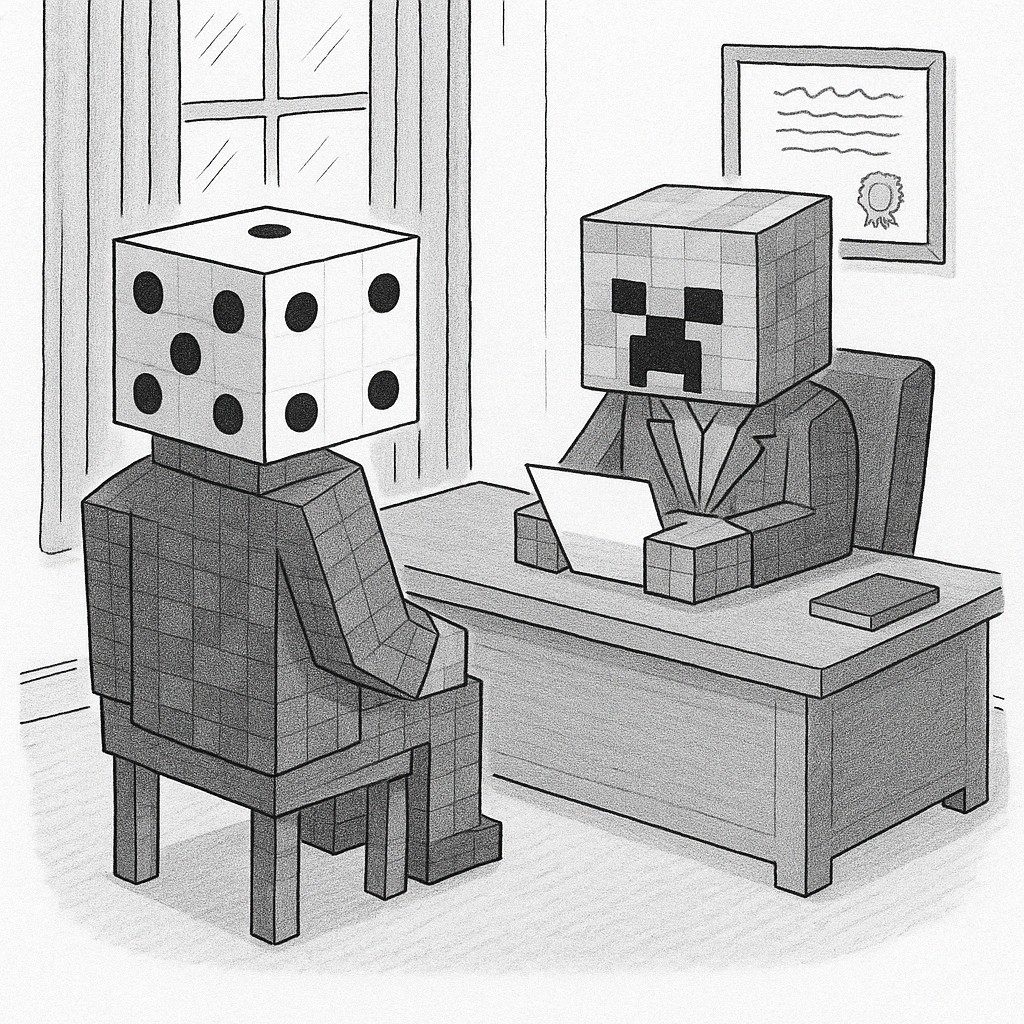
\includegraphics[height=20\baselineskip]{22_MinecraftCreeper/ChatGPT Image Apr 21, 2025, 08_04_30 PM.png}\\
    {\small\textit{Your resume is... interesting. It mentions 'extensive experience in probability determination'?}}
\end{center}
